\chapter{Experimentelle Modalanalyse des Modellflugzeugs}
\label{sec: Hauptkapitel 1}

\section{Aufgabenstellung}
%=========================
    % Grundsätzliches Ziel
    %---------------------
    Bei dieser Laboraufgabe sollen die tieffrequenten Schwingungsmoden des
    Modellflugzeugs bestimmt werden. Die Bestimmung der Moden soll mittels
    experimenteller Modalanalyse durchgeführt werden.
    \\
    %----------------------------------------------------------------------------

    % Ausdetaillierung
    %-----------------
    \noindent
    Es soll dabei bei der Bestimmung der Übertragungsfunktionen kein fertiger
    FRF-Block von Labview verwendet werden. Stattdessen sollen die
    Übertragungsfunktionen durch Division des gemessenen Ausgangs- durch
    Eingangssignals bestimmt werden.
%================================================================================

\section{Versuchsaufbau}
%=======================
    % Diskretisierung des Fliegers
    %-----------------------------
    Da die Messung nur an jeweils einzelnen Punkten durchgeführt werden kann,
    wird in einem ersten Schritt der Modllflieger diskretisiert. Die Messpunkte
    werden dabei mittels Klebenband gekennzeichnet und über Nummern
    unterschieden. Bei der Diskretisierung wird das Modellflugzeug in 3 Bereiche
    unterteilt.
    %----------------------------------------------------------------------------

    % Tab. - Diskretisierung
    %-----------------------
    \begin{table}[h]
        \centering
        \begin{tabular}{|l|c|c|}
            \hline
            \textbf{Bereich} &   \textbf{Schriftfarbe}    &   \textbf{Anzahl der Messpunkte}   \\
            \hline \hline
            vorderer Tragflügel &   rot &   5   \\
            \hline
            Rumpf   &   grün    &   3   \\
            \hline
            hintere Flosse  &   blau    &   2   \\
            \hline
        \end{tabular}
        \caption{Diskretisierung des Modellflugzeugs}
        \label{tab: Fliegerdiskretisierung}
    \end{table}
    %----------------------------------------------------------------------------

    \noindent
    Das diskretisierte Modellflugzeug ist in Abbildung
    \ref{fig: Flieger_diskretisiert} zu sehen.

    % Bild - Diskretisiertes Modellflugzeug
    %--------------------------------------
    \begin{figure}[H]
        \centering
        \includegraphics[width=0.95\textwidth]{Flieger_diskretisiert_Comp.png}
        \caption{diskretisiertes Modellflugzeug}
        \label{fig: Flieger_diskretisiert}
    \end{figure}

    % Bildbeschreibung
    %-----------------
    \noindent
    In Abbildung \ref{fig: Flieger_diskretisiert} sind nur 2 grün beschriftete
    Messpunkte für den Rumpf zu sehen. Das liegt daran, dass der rot markierte
    Punkt 3 des vorderen Tragflügels auch für die Rumpfmessungen herangezogen
    wird.
    \\
    %----------------------------------------------------------------------------

    % Versuchsdurchführung
    %---------------------
    \noindent
    Um die tieffrequenten Moden des Fliegers zu bestimmen, muss in einem ersten
    Schritt die Übertragungsfunktionenmatrix bestimmt werden. Dazu werden
    Messungen mit dem Impulshammer durchgeführt, bei denen ein
    Beschleunigungssignal aufgenommen wird. Es wird dabei die Methode Roving
    Hammer verwendet. Der Beschleunigungssensor bleibt somit immer an Position
    \glqq 5 rot\grqq \hspace{0.05cm} am vorderen Tragflügel (siehe Abbildung
    \ref{fig: Flieger_diskretisiert}).
    %----------------------------------------------------------------------------

    % Verwendete Geräte
    %------------------
    \noindent
    Die verwendeten Messgeräte sind in Tabelle \ref{tab: Geräteliste_EMA}
    angeführt.

    \begin{table}[H]
        \centering
        \begin{tabular}{|l|l|l|}
            \hline
            \textbf{Gerät}  &   \textbf{Seriennummer}   &   \textbf{Sensordaten} \\
            \hline \hline
            Beschleunigungssensor & ... & ... \\
            \hline
            Impulshammer & ... & ... \\
            \hline
            Messkarte & ... & ... \\
            \hline
        \end{tabular}
        \caption{Geräteliste - Experimentelle Modalanalyse}
        \label{tab: Geräteliste_EMA}
    \end{table}    
%================================================================================

\section{Ergebnisse}
%===================
    % Berechnen der Übertragungsfunktion
    %-----------------------------------
    Die Berechnung der Übertragungsfunktionen erfolgt über ein Python-Skript.
    Dieses liest die Messergebnisse, die mit Labview in ein  Excelfile
    gespeichert wurden ein, transformiert diese in den Frequenzbereich und
    bestimmt dann die Übertragungsfunktion. Anschließend werden die Ergebnisse
    wieder in ein Excelfile rausgeschrieben.
    \\
    %----------------------------------------------------------------------------

    % Bestimmen der Moden
    %--------------------
    \noindent
    Die Moden des Flugzeugs können nun durch Betrachtung der
    Übertragungsfunktionen bestimmt werden. Um die Frequenzlage zu bestimmen,
    wird der Bereich, in dem im Plot der Übertragungsfunktionen ein Mode
    vermutetet wird, genauer betrachtet. Im Falle der Amplitude wird ein
    Maximum in diesem Bereich gesucht. Bei Betrachtung des Imaginärteils wird der
    größte Absolutwert im Bereich verwendet und bei Betrachtung des Realteils
    wird ein Nulldurchgang gesucht. Dieser Vorgang wird für jede
    Übertragungsfunktion durchgeführt. Die sich dadurch ergebenden
    Frequenzlagen werden zu einem Mittelwert zusammengefasst. Somit ergeben sich
    3 gemittelte Frequenzlagen der Moden, einmal aus der Amplitude, einmal aus 
    dem Imaginärteil und aus dem Realteil. Im Anschluss werden diese 3
    Mittelwerte erneut zu einem Mittelwert zusammengefasst. Es ergeben sich
    folgende, tieffrequente Moden des Modellflugzeugs:
    %----------------------------------------------------------------------------

    % Tabelle mit den Moden
    %----------------------
    \begin{table}[H]
        \centering
        \begin{tabular}{|c|c|}
            \hline
            \textbf{Mode}   &   \textbf{Frequenzlage [Hz]}  \\
            \hline \hline
            Mode 1  &   5.048 \\
            \hline
            Mode 2  &   20.02 \\
            \hline
            Mode 3  &   46.34 \\
            \hline
            Mode 4  &   49.707 \\
            \hline            
        \end{tabular}
        \caption{Frequenzlage der tieffrequenten Moden}
        \label{tab: Frequenzlage_Moden}
    \end{table}
    %----------------------------------------------------------------------------

    % Amplitudenplot
    %---------------
    \noindent
    Diese 4 Moden decken sich auch gut mit den Betrachtungen des Plots der
    Amplituden der Übertragungsfunktionen (siehe Abbildung
    \ref{fig: Amplitudenplot}).

    % Bild - Amplitudenplot
    %----------------------
    \begin{figure}[H]
        \centering
        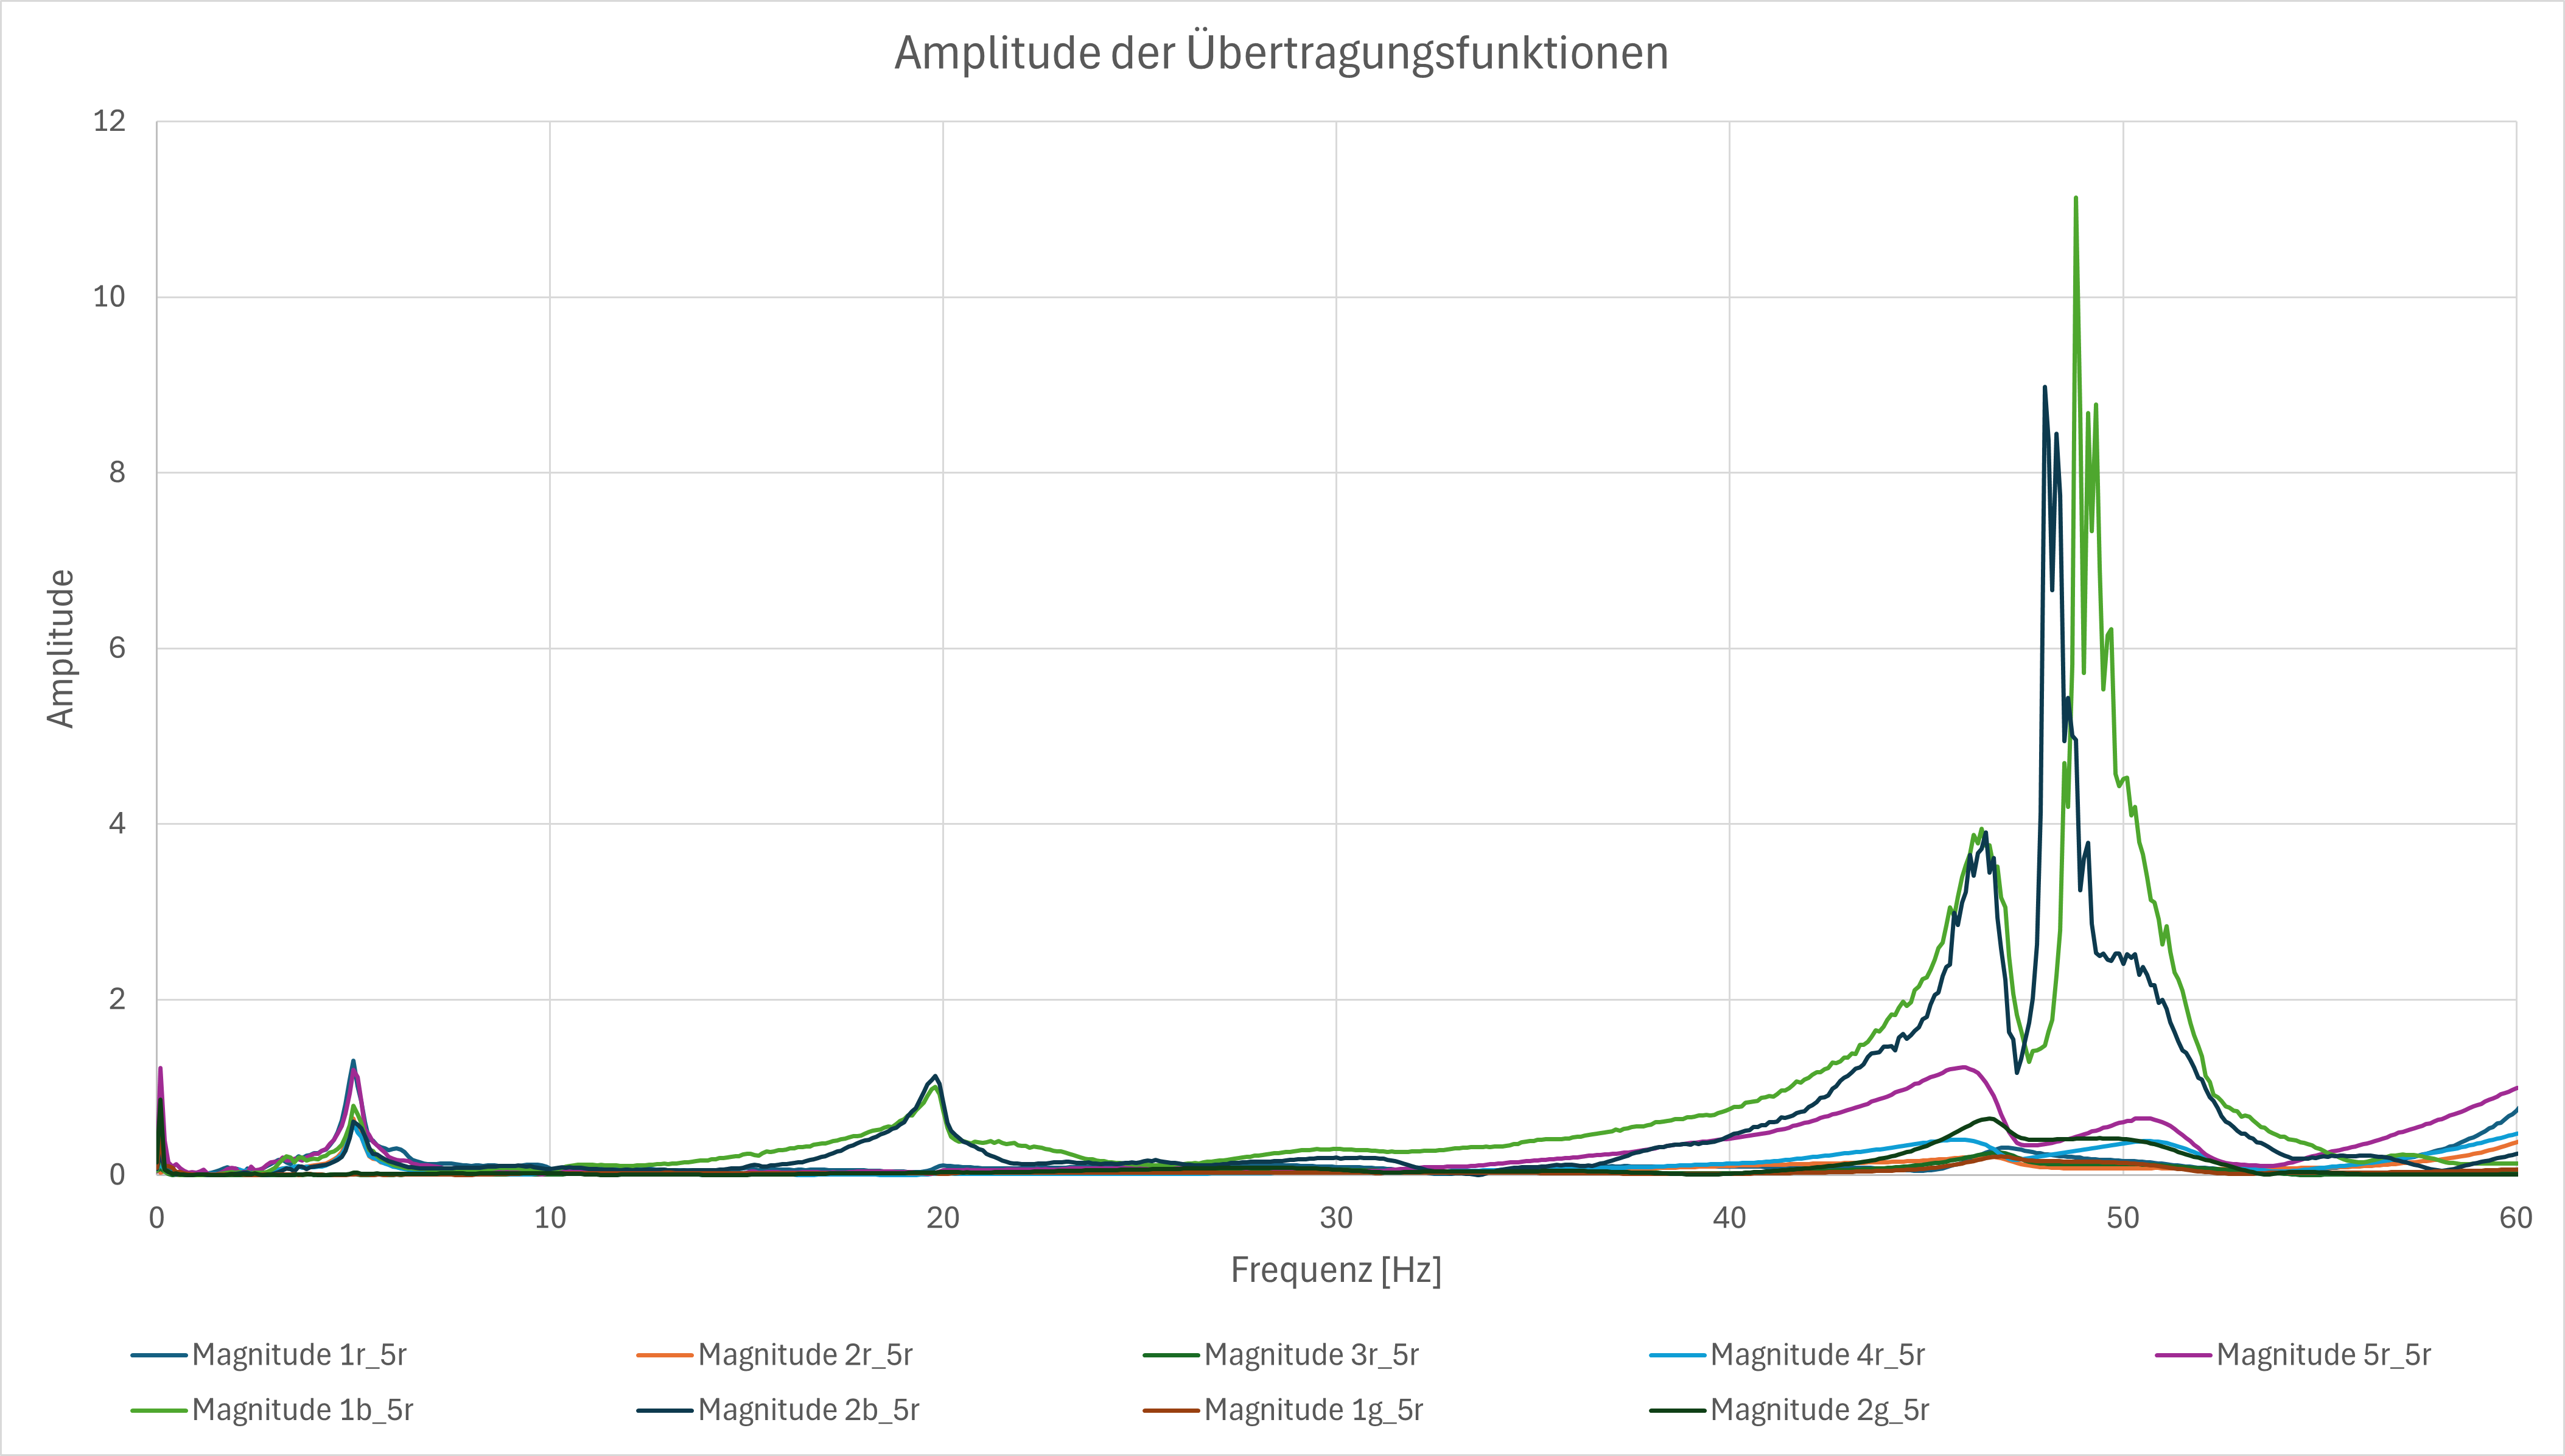
\includegraphics[width=0.95\textwidth]{Amplitudenplot.png}
        \caption{Amplitude der Übertragungsfunktionen}
        \label{fig: Amplitudenplot}
    \end{figure}
    %----------------------------------------------------------------------------

    % Modeformen
    %-----------
    \noindent
    Des Weiteren können die Modformen bestimmt werden. Dazu wird der
    Imaginärteil der Übertragungsfunktionen herangezogen. Mit einem
    Python-Skript (siehe Anhang \ref{sec: Anhang_EMA}) wird ein Drahtmodell
    generiert, das die Modform widergibt. In den Abbildungen
    \ref{fig: Modeform_1} bis \ref{fig: Modeform_4} sind die Modformen
    der ersten 4 Moden zu sehen.

    % Bild - Modform 1
    %-----------------
    \begin{figure}[H]
        \centering
        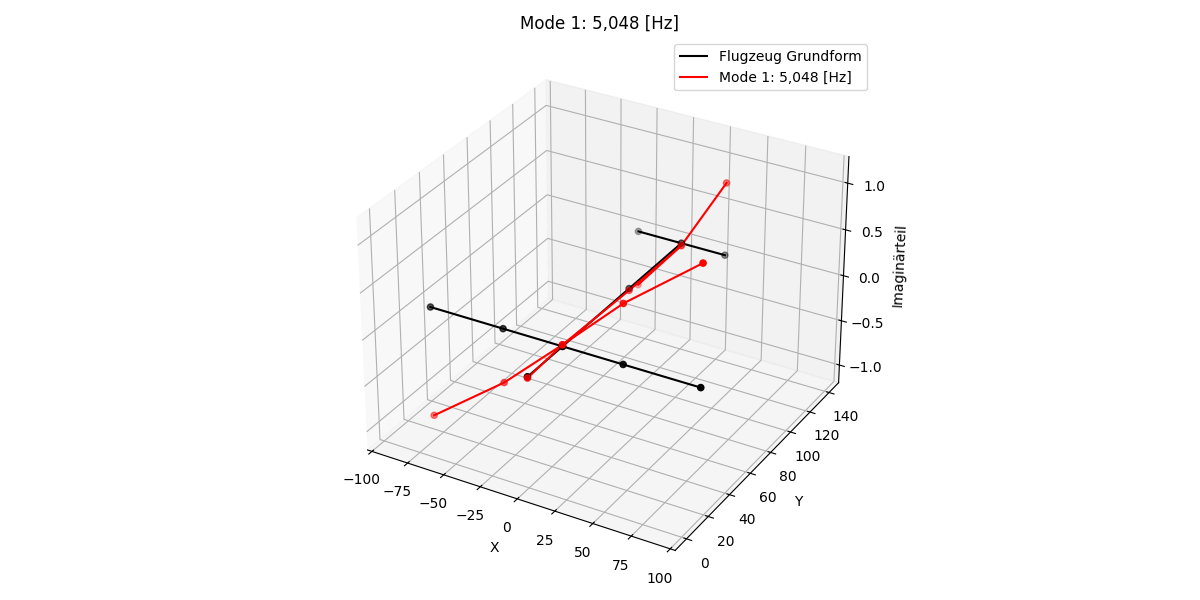
\includegraphics[width=1\textwidth]{Modeform_1.png}
        \caption{Modeform des 1. Moden}
        \label{fig: Modeform_1}
    \end{figure}

    % Bild - Modform 2
    %-----------------
    \begin{figure}[H]
        \centering
        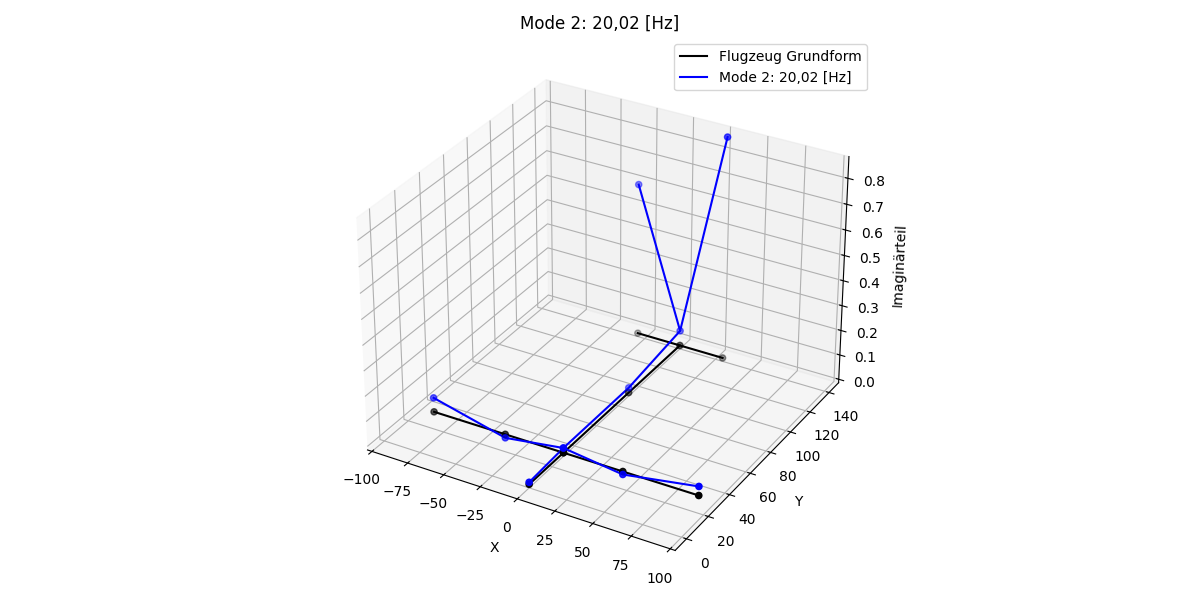
\includegraphics[width=1\textwidth]{Modeform_2.png}
        \caption{Modeform des 2. Moden}
        \label{fig: Modeform_2}
    \end{figure}

    % Bild - Modform 3
    %-----------------
    \begin{figure}[H]
        \centering
        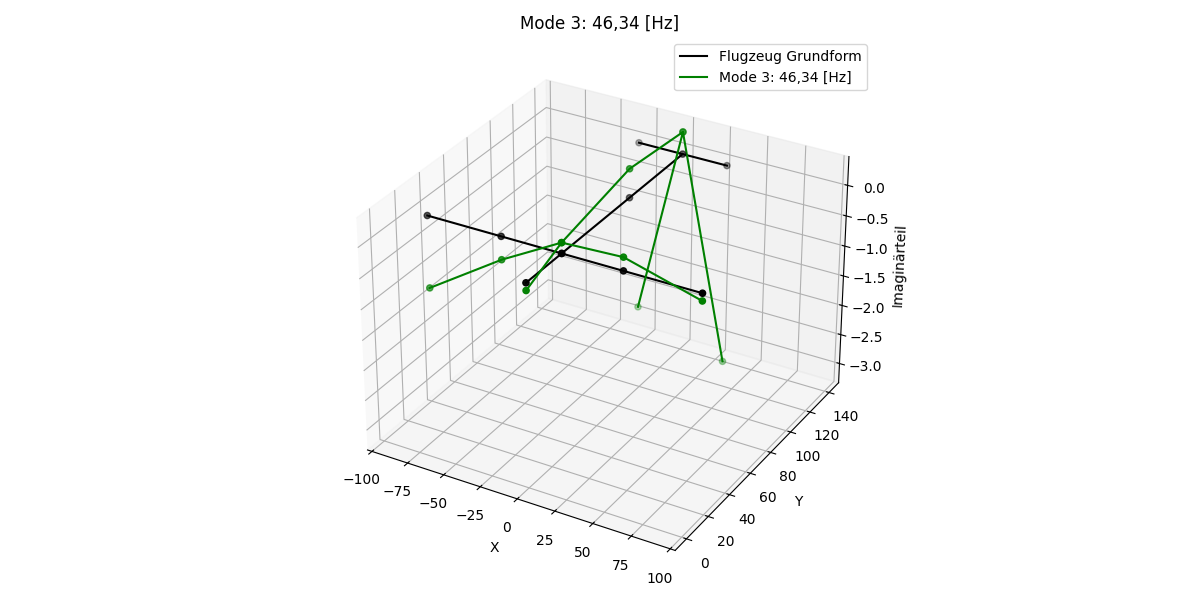
\includegraphics[width=1\textwidth]{Modeform_3.png}
        \caption{Modeform des 3. Moden}
        \label{fig: Modeform_3}
    \end{figure}

    % Bild - Modform 4
    %-----------------
    \begin{figure}[H]
        \centering
        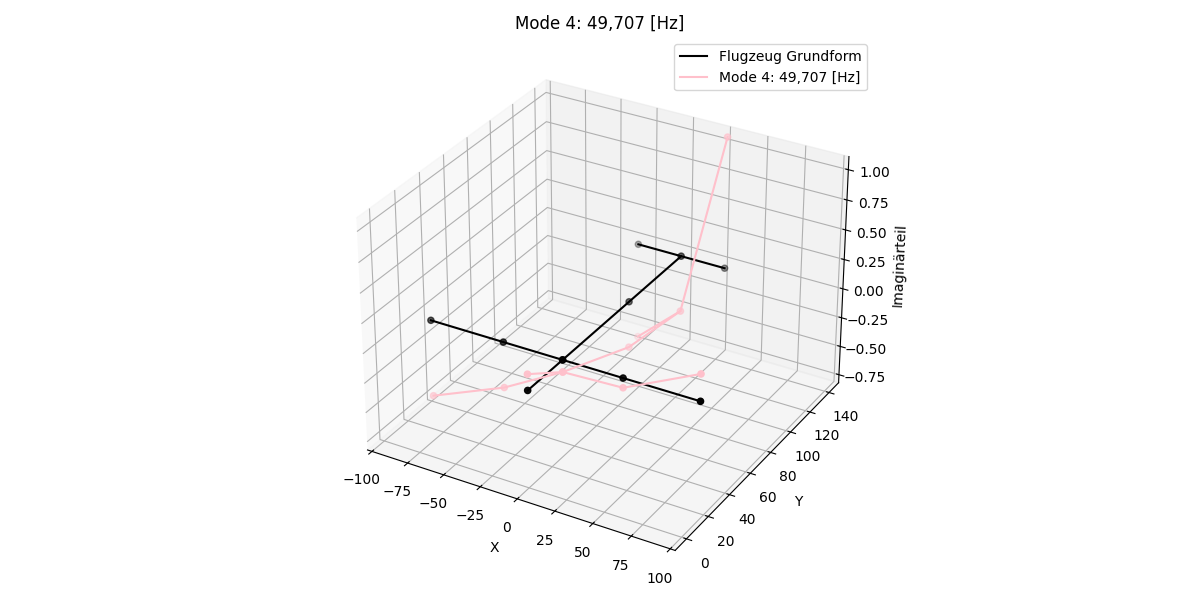
\includegraphics[width=1\textwidth]{Modeform_4.png}
        \caption{Modeform des 4. Moden}
        \label{fig: Modeform_4}
    \end{figure}
    %----------------------------------------------------------------------------

    % Interpretation der Modformen
    %-----------------------------
    \noindent
    In Abbildung \ref{fig: Modeform_1} ist gut zu sehen, dass es sich beim 1.
    Mode des Modellflugzeugs um einen Starrkörpermoden handelt, bei dem der
    Flieger um die Rumpfachse gedreht wird. Auch der 2. Mode
    (siehe Abbildung \ref{fig: Modeform_2}) lässt sich gut als
    \glqq Vogelmode\grqq \hspace{0.05cm} identifizieren. Die Formen des 3. und 4.
    Moden müssen jedoch mit einer gewissen Skepsis betrachtet werden. Wie aus
    Abbildung \ref{fig: Amplitudenplot} hervorgeht, liegen diese beiden Moden
    relativ nahe beieinander. Da zur Bestimmung der Modeform gut separierte
    Moden angenommen werden, ist nicht klar, ob diese Annahme auch für den 3.
    und 4. Moden zulässig ist. Somit kann nicht garantiert werden, dass die in
    den Abbildungen \ref{fig: Modeform_3} und \ref{fig: Modeform_4}
    dargestellten Modeformen auch tatsächlich nur von einem einzelnen Mode
    herrühren. Vielmehr muss angenommen werden, dass es sich um einen
    kombinierten Einfluss von Mode 3 und Mode 4 handelt.